\documentclass[main.tex]{subfiles}
\begin{document}
	\section{Používateľská príručka}
		\begin{multicols}{2}
			\subsection{Používateľské rozhranie}
			V krátkosti opíšeme časti používateľského rozhrania. Po spustení programu sa zobrazí okno na \cref{fig:GUIPrveOkno}. Vysvetlenie jednotlivých nastavení je v \cref{tab:GUIVysvetlenieNastaveni}. Začatím merania, je potrebné vytvoriť spojenie so zariadením. Najprv je treba prepnúť sa do okna $Protocol$ vyznačené na \cref{fig:GUIPrveOkno}. Po prepnutí sa zobrazia nastavenia komunikácie na \cref{fig:GUINastaveniaKomunikacie}, kde je potrebné vybrať správny sériový port, na ktorom je zariadenie pripojené a nastaviť vhodnú prenosovú rýchlosť. Po nastavení týchto parametrov je treba kliknúť na tlačidlo $Connect$ a počkať ($~1$sec) kým sa nezmení indikátor stavu spojenia na zelenú alebo červenú. Spojenie prebehlo úspešne v prípade zelenej farby indikátora stavu spojenia.
			
			Meranie sa potom spúšťa tlačidlom $Measure$, ktorého stlačením sa zašlú aktuálne nastavenia do mikropočítača. V prípade, že žiadame aby sa citlivosť a posunutie kanálu aplikovala automaticky, je možné zaškrtnúť checkbox $autoupdate$. Zaškrtnutím $autoupdate$ sa s frekvenciou $10HZ$ budú do mikropočítača posielať požiadavky o úpravu transformačných parametrov.  
			
			
		\end{multicols}
	
		\begin{figure}[h!]
			\centering
			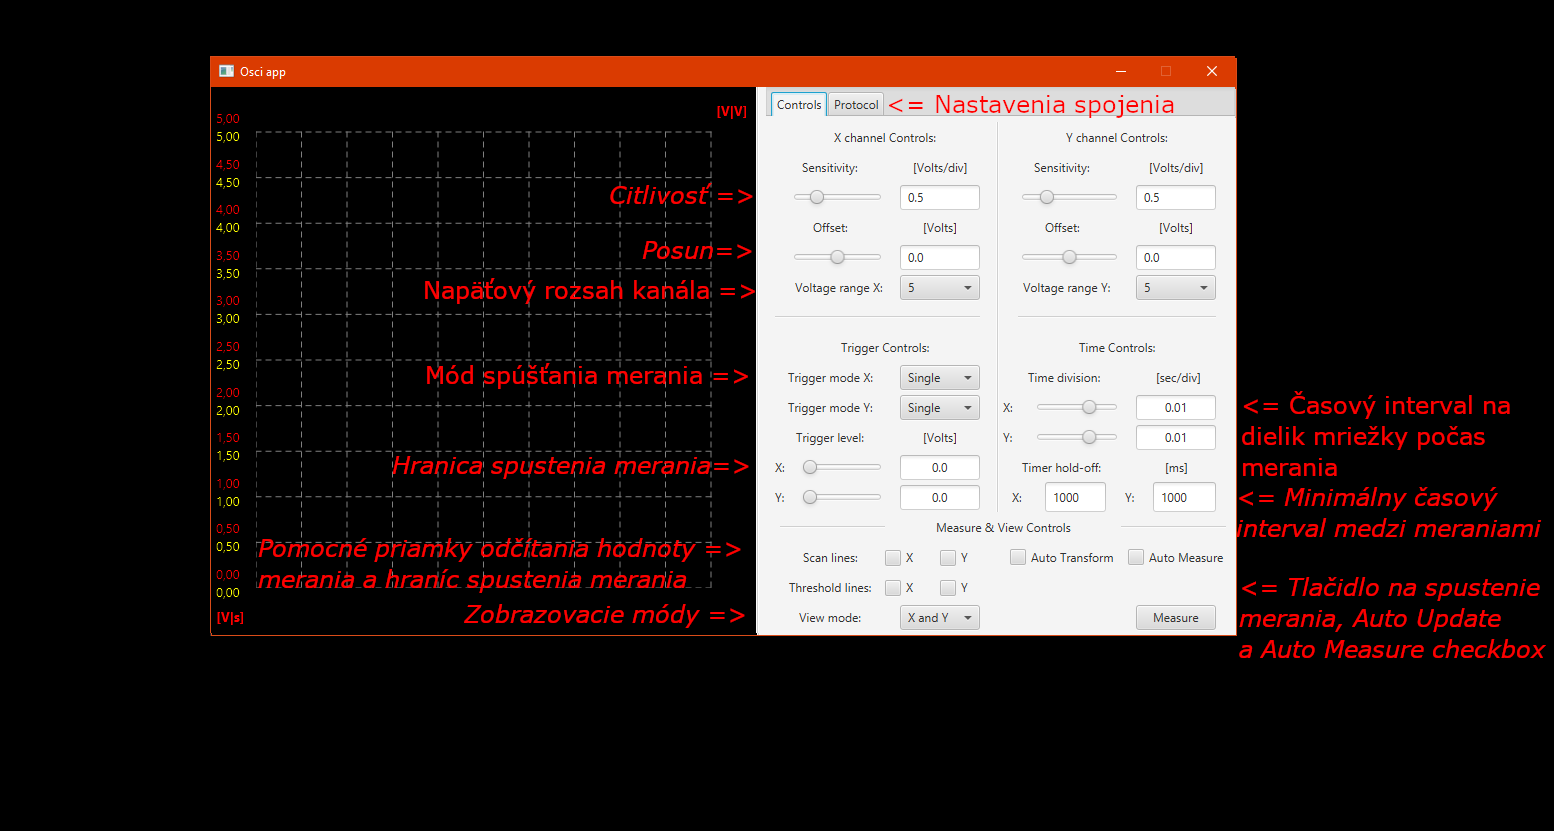
\includegraphics[width=\linewidth]{../Obrazky/GUIPrveOkno}
			\caption{Úvodné okno používateľského rozhrania}
			\label{fig:GUIPrveOkno}
		\end{figure}
	
		\begin{table}
			\begin{tabular}{p{5cm}|c|p{5cm}}
				Nastavenie & Jednotky & Vysvetlenie \\
				\hline
				Citlivosť & V/dielik mriežky & Určuje s akou citlivosťou sa budú dáta zobrazovať \\
				Posun & V & Udáva posun, ktorý je pripočítaný k nameraným dátam pri zobrazovaní \\ 
				Napäťový rozsah kanála & V & Určuje nastavenie vstupného deliča napätia \\ 
				Metódy spúšťania merania & - & Buď $Single$ - vykonanie jedného merania, alebo $Continous$ - pravidelné opakovanie merania\\ 
				Hranica spustenia merania & - & Určuje hranicu napätia, prekročenie ktorej spustí meranie\\ 
				Časový interval na dielik mriežky & sec & Určuje periódu vzorkovania pri meraní \\
				Minimálny časový interval medzi meraniami & msec & Určuje minimálny časový interval medzi meraniami v $Continous$ móde \\
			\end{tabular}
			\caption{Vysvetlenie nastavení}
			\label{tab:GUIVysvetlenieNastaveni}
		\end{table}
		\begin{figure}
			\centering
			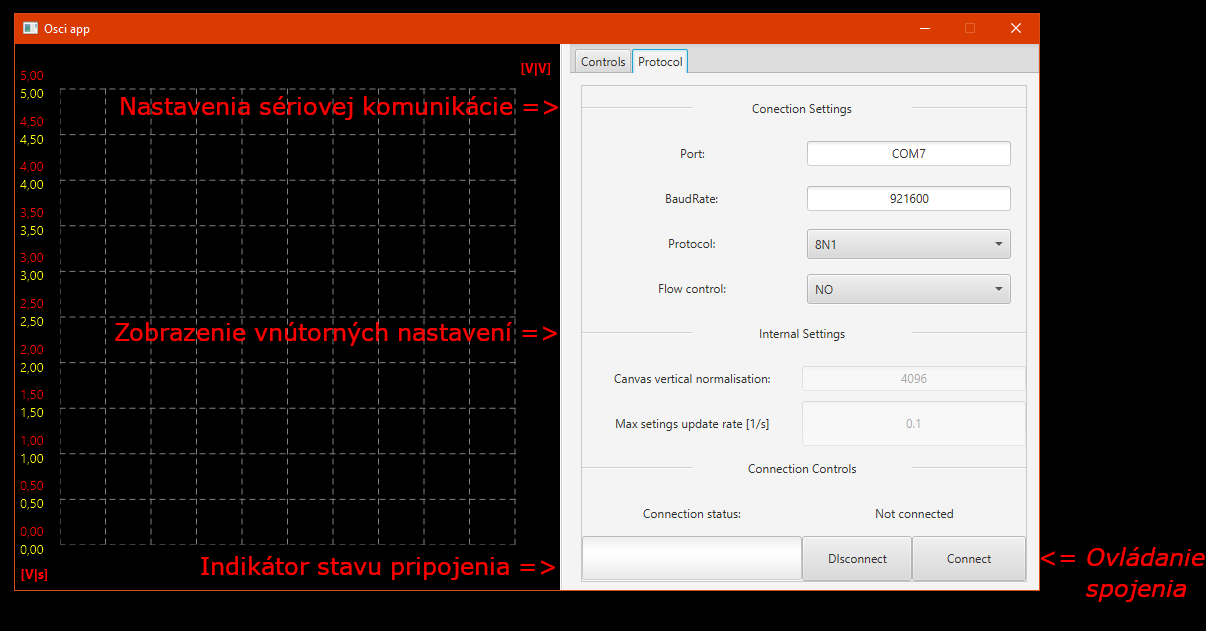
\includegraphics[width=\linewidth]{../Obrazky/GUINastaveniaKomunikacie}
			\caption{Okno nastavení komunikácie}
			\label{fig:GUINastaveniaKomunikacie}
		\end{figure}
		\FloatBarrier
		\begin{multicols}{2}
			\subsection{Spustenie merania}
			\begin{enumerate}
				\item Zapnutie GUI
				\item Prepnutie do záložky Protocol
				\item Nastavenie parametrov protokolu 
				\item Kliknutie na tlačidlo Connect
				\item Ak je ProgressBar naľavo zelený, spojenie prebehlo úspešne, inak nie a v takom prípade, je treba znova overiť, či boli zadané parametre správne.
				\item Prepnutie naspäť na záložku Control
				\item Nastavenie parametrov merania
				\item V prípade, že vyžadujeme aj automatickú aktualizáciu parametrov transformácie, tak zaškrtnime CheckBox autoupdate.
				\item Klikneme na tlačidlo Measure
				\item Počkáme, až kým sa naľavo nezobrazia namerané priebehy.
			\end{enumerate}
		\end{multicols}
\end{document}